\documentclass[compress]{beamer}

%--------------------------------------------------------------------------
% Common packages
%--------------------------------------------------------------------------
\usepackage[english]{babel}
\usepackage{pgfpages} % required for notes on second screen
\usepackage{graphicx}

\usepackage{multicol}

\usepackage{tabularx,ragged2e}
\usepackage{booktabs}

%--------------------------------------------------------------------------
% Load theme
%--------------------------------------------------------------------------
\usetheme{hri}

\usepackage{tikz}
\usetikzlibrary{calc,mindmap,backgrounds,positioning}

\graphicspath{{figs/}}

%--------------------------------------------------------------------------
% General presentation settings
%--------------------------------------------------------------------------
\title{From Attention to With-me-ness}
\subtitle{(what a lovely neologism)}
\date{\today}
\author{Séverin Lemaignan}
\institute{Centre for Robotics and Neural Systems\\ {\Medium
Plymouth University}}

%--------------------------------------------------------------------------
% Notes settings
%--------------------------------------------------------------------------
%\setbeameroption{show notes on second screen}

\begin{document}

\licenseframe{https://github.com/severin-lemaignan/hri2016-withmeness-presentation}

\maketitle

\section{Attention tracking}

\begin{frame}[plain]{}
    \begin{center}
     \only<1>{
        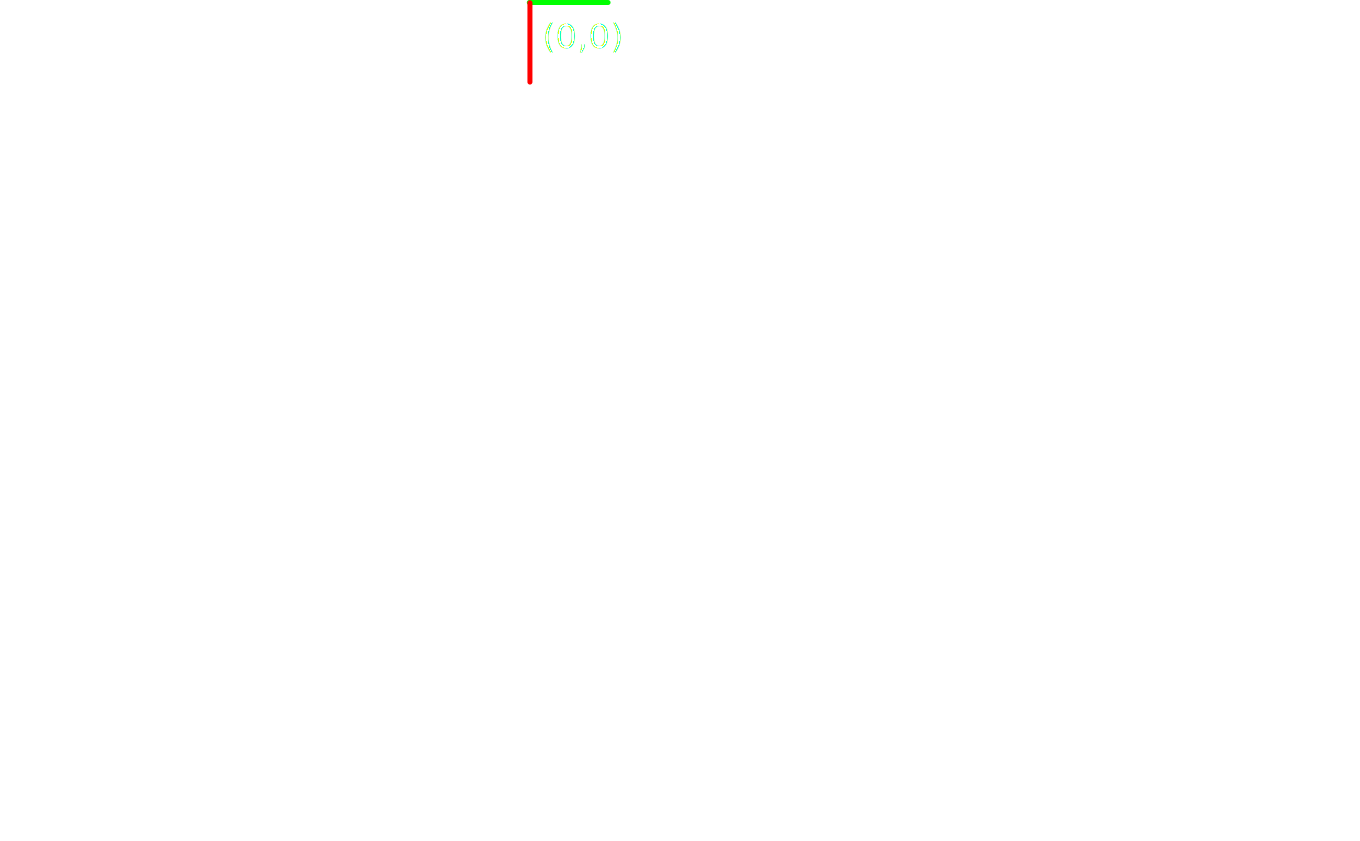
\includegraphics[width=0.8\linewidth]{head_pose0}
    }
     \only<2>{
        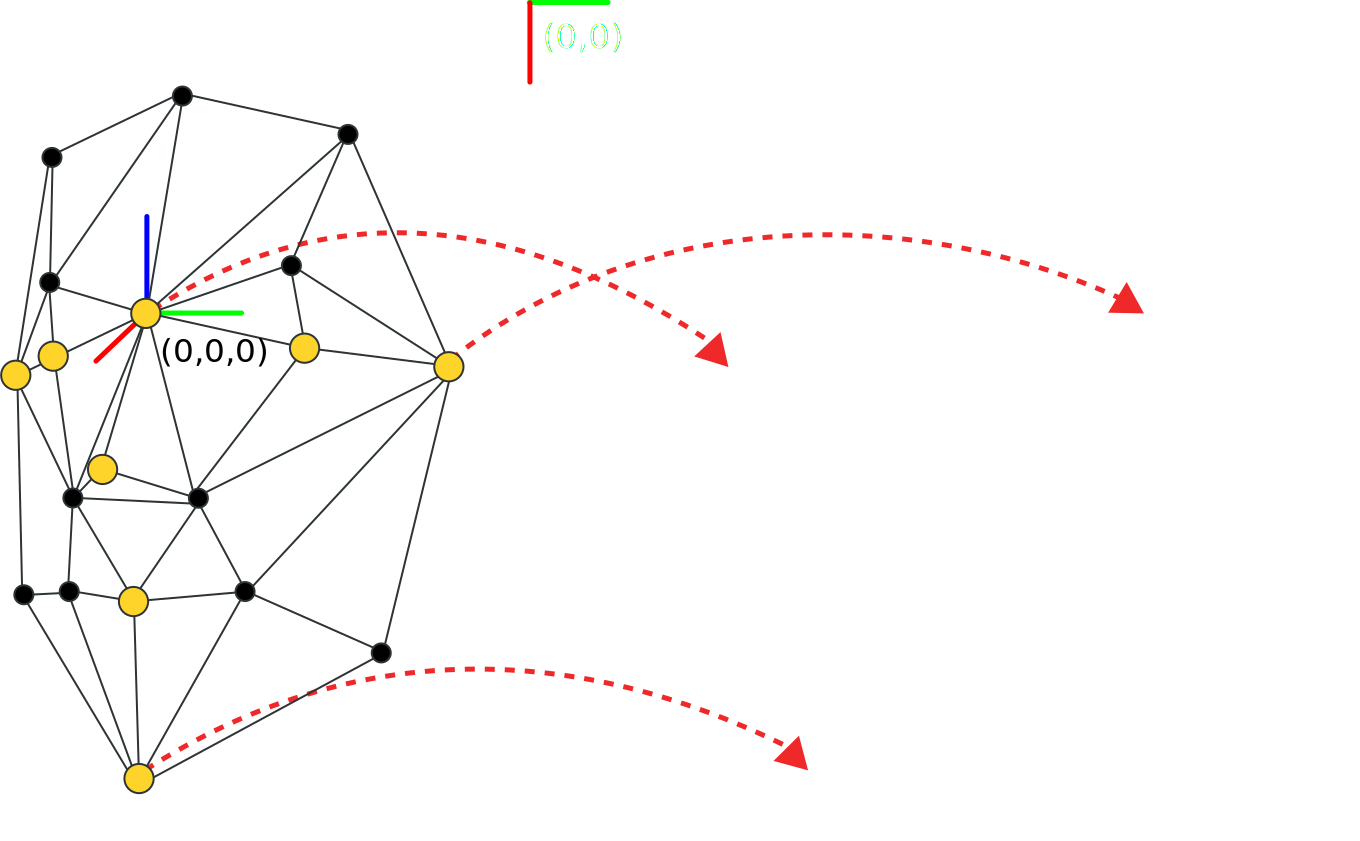
\includegraphics[width=0.8\linewidth]{head_pose}
    }

     \only<3->{
        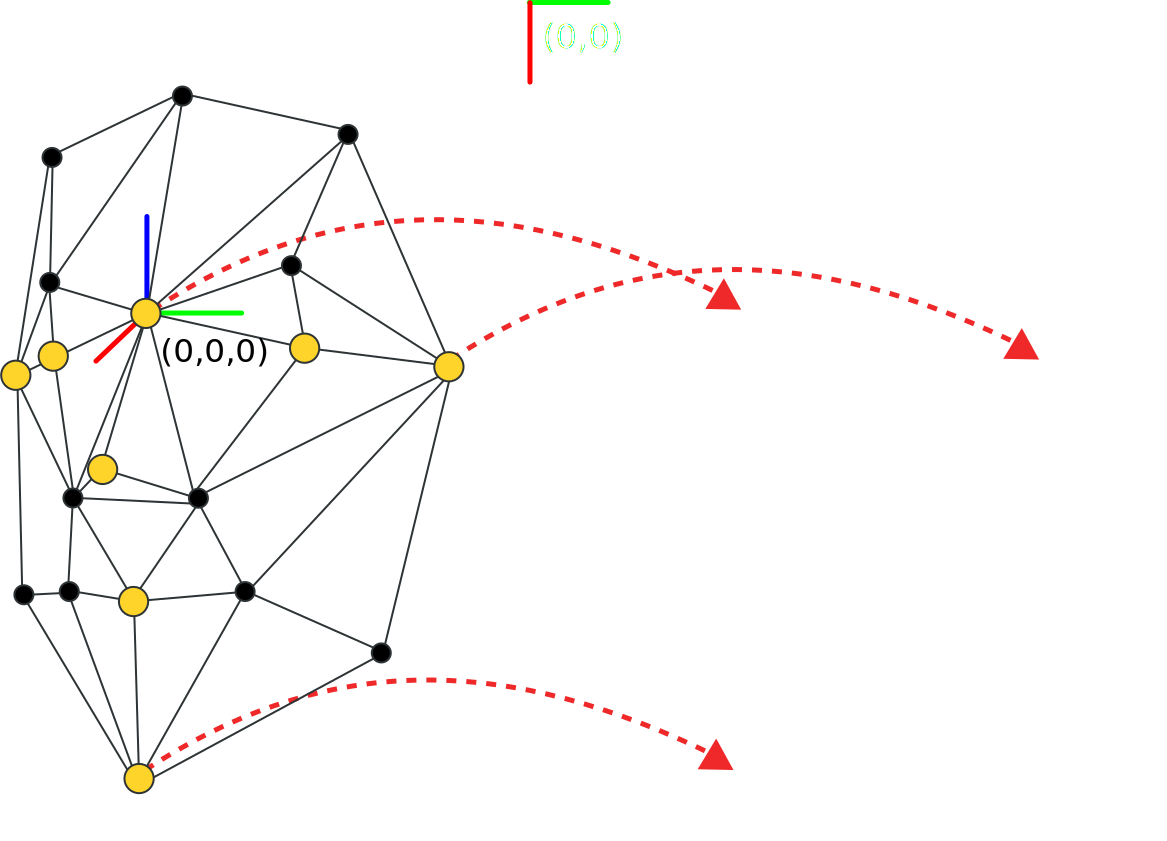
\includegraphics[width=0.8\linewidth]{head_pose2}
    }

    \texttt{dlib}
    \uncover<2->{+ OpenCV}
    \uncover<3->{= \texttt{gazr}

    \url{http://github.com/severin-lemaignan/gazr}}
    \end{center}
\end{frame}


\imageframe[color=black]{head_pose_real_world}

\imageframe[color=black]{field_of_attention0}

\section{Experimental setup}

\imageframe[color=black]{realSetup}
\imageframe{experimental_setup}
\imageframe[color=black]{field_of_attention}

\begin{frame}{How accurate?}
    \begin{center}
        \only<1>{
            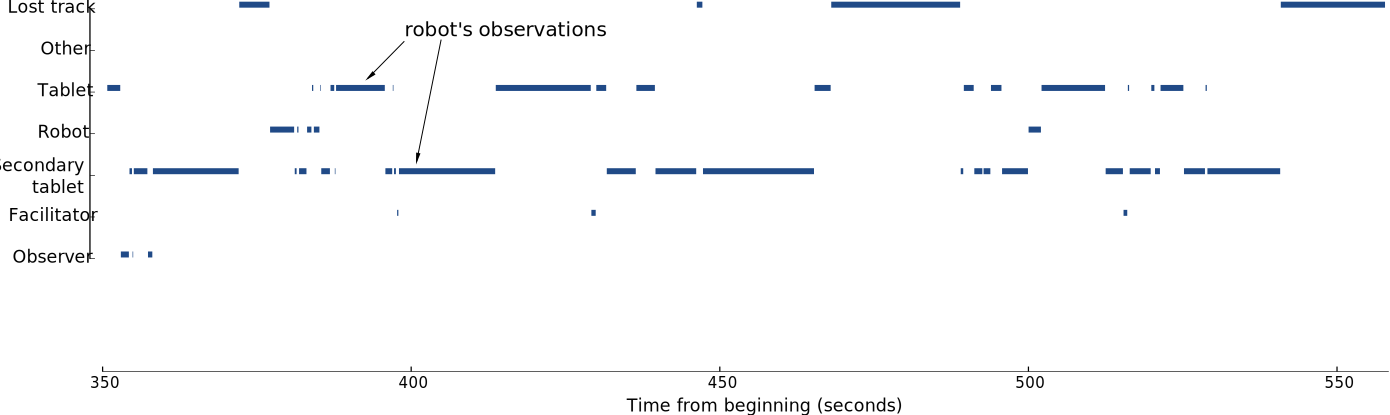
\includegraphics[width=\linewidth]{matches-excerpt0}
        }
        \only<2->{

        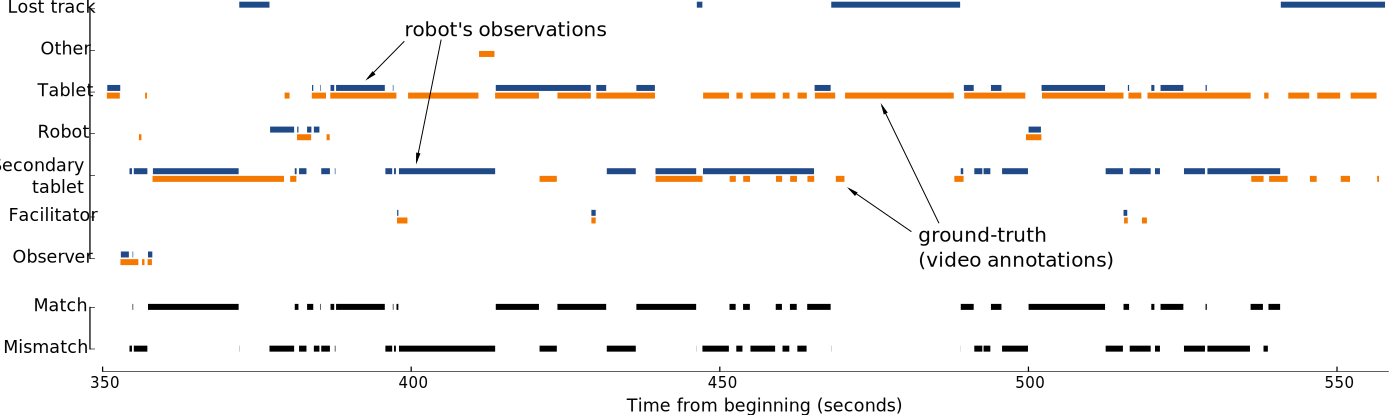
\includegraphics[width=\linewidth]{matches-excerpt}
    }

    \vspace{2em}
\only<1,2>{
    \scriptsize
    \begin{tabular}{p{3.3cm}cccccccc}
        \toprule
        {\Medium Subject} & 1 & 2 & 3 & 4 & 5 & 6 & {\Medium M} & {\it SD} \\
        \midrule
        {\bf Head pose tracking} (\%) & 88.2 & 83.5 & 90.5 & 83.1 & 87.9 & 85.0 & {\Medium 86.4} & {\it 3.0} \\ 
        \bottomrule
    \end{tabular}
}

\uncover<3>{
    \scriptsize
    \begin{tabular}{p{3.3cm}cccccccc}
        \toprule
        {\Medium Subject} & 1 & 2 & 3 & 4 & 5 & 6 & {\Medium M} & {\it SD} \\
        \midrule
        {\bf Head pose tracking} (\%) & 88.2 & 83.5 & 90.5 & 83.1 & 87.9 & 85.0 & {\Medium 86.4} & {\it 3.0} \\ 
        \midrule
        {\bf Agreement} (\%) & 58.9 & 67.1 & 79.2 & 48.3 & 65 & 77.1 & {\Medium 65.9} & {\it 11.5}\\
        {\bf Cohen's $\kappa$} & 0.48 & 0.56 & 0.68 & 0.26 & 0.47 & 0.68 & {\Medium 0.52} & {\it 0.16}\\
        \bottomrule
    \end{tabular}
}
    \vspace{6em}
    \end{center}
\end{frame}

\section{With-me-ness}

\begin{frame}[plain]{}
    \begin{center}
        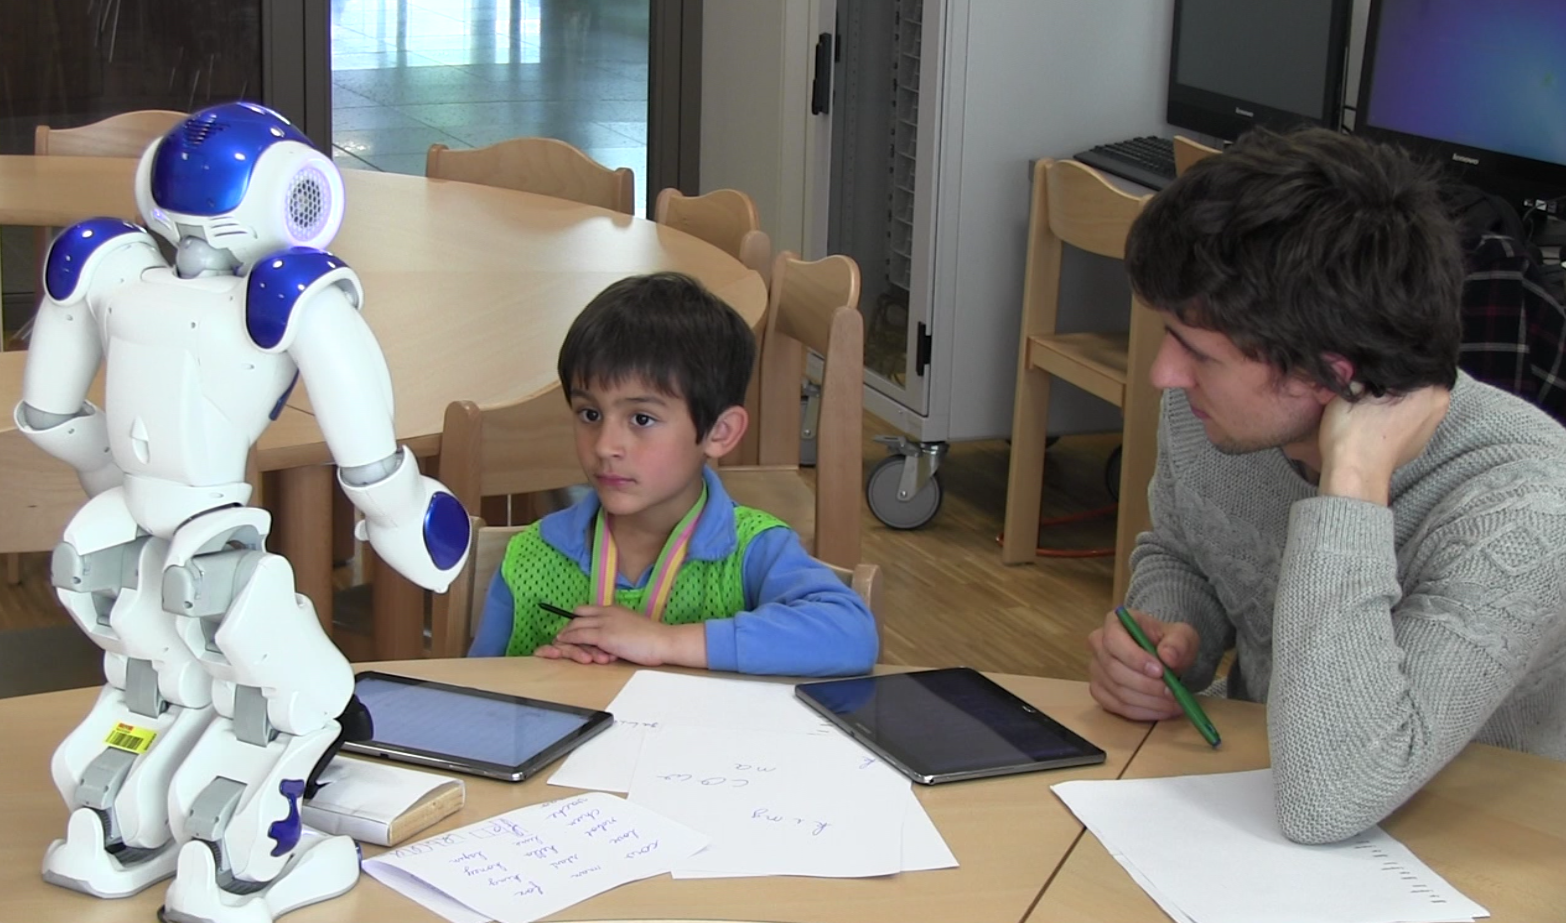
\includegraphics[width=0.8\linewidth]{realSetup}

        \only<1>{
        {\Medium Robot's expectations:}
        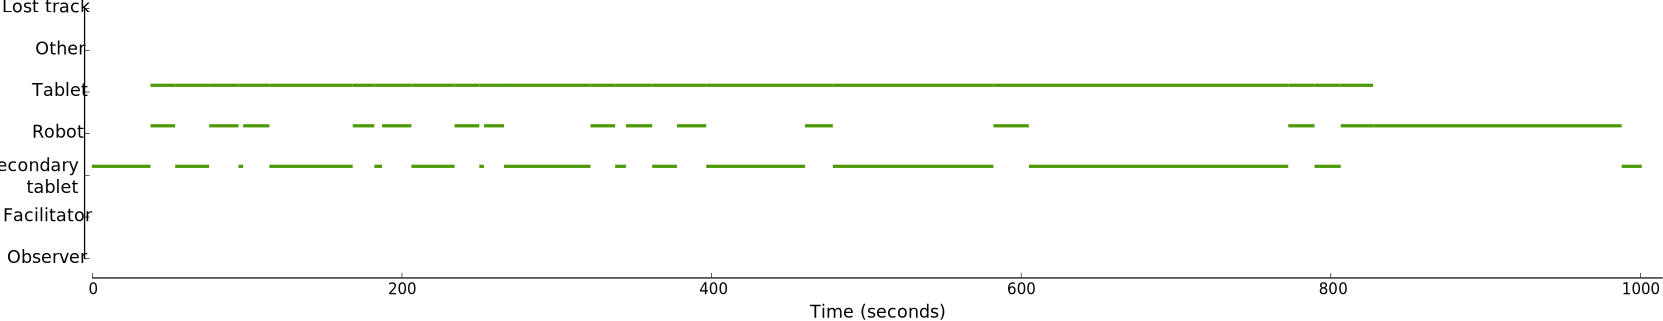
\includegraphics[width=\linewidth]{with-me-ness-expectations}
    }
    \only<2>{
        {\Medium Expectations vs observations:}
        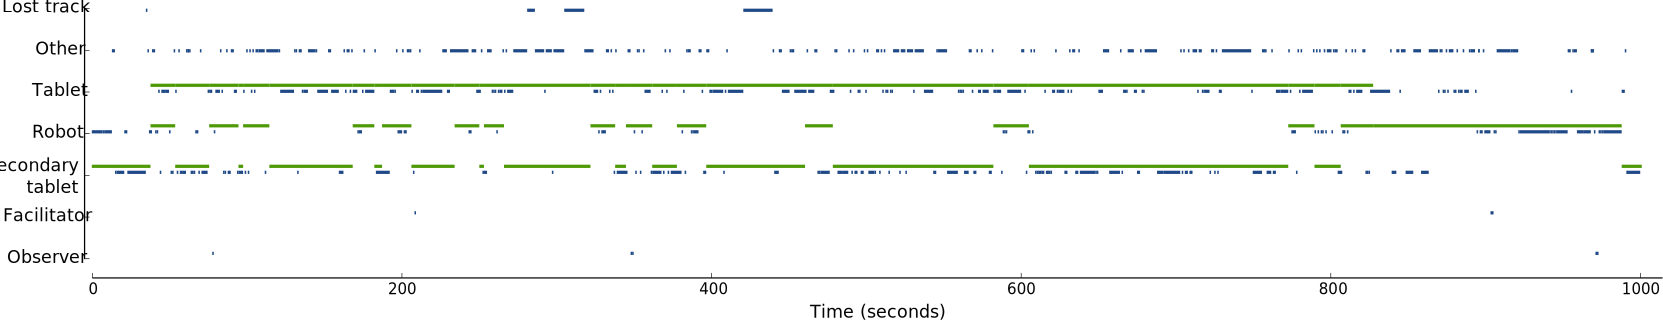
\includegraphics[width=\linewidth]{with-me-ness-expectations-observations}
    }
    \end{center}
\end{frame}

\begin{frame}[fragile]{}
\begin{pythoncode}

def withmeness(startime, endtime):

    withme_duration = expected_duration = 0
    dt = 0.1 #typically in sec

    for t in range(starttime, endtime, dt):
        task = task_at(t)
        expected_foci = expected_foci(task)
        focus = user_focus_at(t)

        if task and expected_foci and focus:
            if focus in expected_foci:
                withme_duration += dt

            expected_duration += dt

    return withme_duration / expected_duration

\end{pythoncode}

\end{frame}

\imageframe[scale=0.95]{with-me-ness-robot}
{\fullbackground[scale=0.95]{with-me-ness-groundtruth}
    \begin{frame}{}
        \vspace{6cm}
        \begin{center}
        $r(973) = 0.58, p < .001$
            
        \end{center}
    \end{frame}

}

\begin{frame}{Expected focus}

    \centering
    \python{def expected_foci(task)}?

    \uncover<2->{
        \begin{multicols}{2}
           \scriptsize 
           \begin{tabular}{p{2.5cm}p{2.5cm}}
            \toprule
            {\Medium Interaction Phase} & {\Medium Expected targets} \\
            \midrule
            Presentation & {\sf robot} \\ 
            \midrule
            Waiting for word & {\sf secondary tablet} \\ 
            \midrule
            Writing word & {\sf tablet}\newline {\sf robot} \\ 
            \midrule
            Waiting for feedback & {\sf tablet}\newline {\sf secondary tablet} \\ 
            \midrule
            Story telling & {\sf robot} \\ 
            \midrule
            Bye & {\sf robot} \\ 
            \bottomrule
        \end{tabular}

            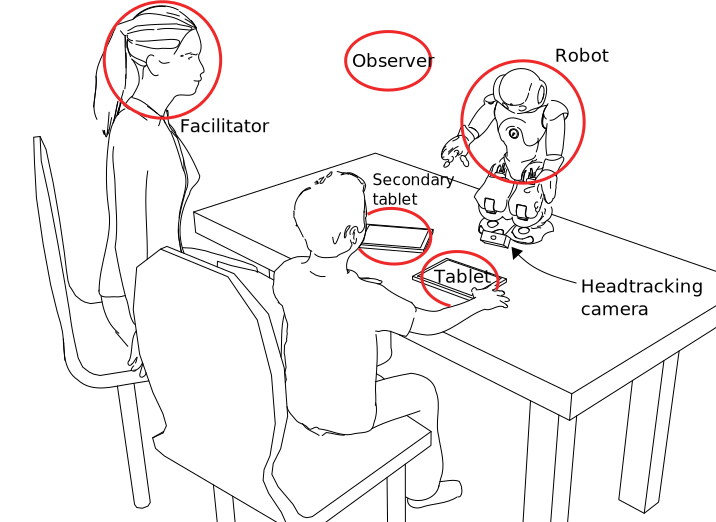
\includegraphics[width=0.95\columnwidth]{experimental_setup}
        \end{multicols}
    }
    \uncover<3>{
        Resulting with-me-ness value {\Medium very sensitive to this mapping}\\
        With-me-ness is a {\Medium relative metric}!
    }
\end{frame}

\section{What does it says about the interaction?}
\imageframe[scale=0.95]{with-me-ness}


\end{document}






